\section{Введение}
\label{sec:Chapter0} \index{Chapter0}

\sloppy

Изменение семантики программы посредством манипуляции ее бинарным кодом является распространенной техникой, используемой в современной разработке. Она используется для добавления к существующему проекту элементов рефлексии или имплементации парадигм аспектно-ориентированного программирования (далее АОП). Зачастую, целью подобных изменений является решение существующих проблем традиционного объектно-ориентированного программирования (далее ООП). Несмотря на то, что применение ООП позволяет увеличить продуктивность разработки за счет переиспользования существующих компонент посредством таких механизмов как полиморфизм и наследование, соблюдение этих принципов не всегда возможно. Например в проектах, в которых невозможно реализовать централизованную стратегию разработки и развития всех компонент, таких как внешние библиотеки. Конечный пользователь не имеет контроля над совместимостью компонент из разных библиотек, а также не всегда имеет доступ к исходному коду, что приводит к проблеме обеспечения функциональной совместимости (интероперабельности) между компонентами. Для решения этой проблемы ООП предлагает написание классов-оберток, которые бы обеспечивали интерфейсную совместимость. Данный подход приводит к проблемам поддержки кодовой базы, а также обеспечения выполнения контрактов между компонентами. Бинарная манипуляция является альтернативным решением проблем интероперабельности. Вместо того, чтобы создавать новые классы-обертки, пользователь может модифицировать оригинальные определения в библиотеке \cite{bca}. Изменения происходят на стороне пользователя после поставки компоненты, и не требуют доступа к исходному коду.

Помимо обеспечения интероперабельности между компонентами, бинарная манипуляция также применяется для обеспечения принципа разделения обязанностей, являющегося важной частью АОП. Соблюдение этого принципа заключается в отделении разработки функциональной части приложения от имплементации нефункциональных контрактов, таких как обеспечение безопасности, поддержка единой модели распространения приложения и других. Для достижения этой цели недостаточно простого изменения интерфейсов или иерархии классов, и необходимо иметь инструменты для модификации тел уже существующих функций \cite{tanter2002}.

Помимо упомянутых выше, существует еще множество областей применения бинарной инструментации. Ниже приведен более подробный разбор уже существующих задач, а также рассмотрены некоторые другие области применения данной техники.

\subsection{Интероперабельность}

Интероперабельность - это способность двух или более компонент программного обеспечения работать вместе несмотря на различия в языке, интерфейсе или исполняющей платформе \cite{malone2014}. В рамках данной работы остановимся на рассмотрении кросс-интерфейсной интероперабельности и того, как задача бинарной манипуляции связана с ней.

Существует два основных механизма для реализации интероперабельности: стандартизация интерфейсов (Interface Standartization) и интерфейсный мост (Interface Bridging). Первый подход заключается в создании единого интерфейса и последующего приведения интерфейсов участников взаимодействия к нему. Второй подход состоит в создании взаимно однозначного соответствия между интерфейсами всех участников взаимодействия \cite{wegner1996}. Стандартизация интерфейсов зачастую является предпочтительным решением, поскольку является наиболее масштабируемым. Действительно, для данного подхода нужно построить всего $n + m$ соответствий, где $n$ - число интерфейсов первого участника, и $m$ - число интерфейсов второго участника взаимодействия. Для второго подхода число соответствий будет равно $m * n$. Недостатком же стандартизации интерфейсов является то, что она значительно усложняет дальнейшее расширение интерфейсов, а также поддержку новых функциональностей, отсутствующих в языке на момент стандартизации интерфейсов. Промышленным примером системы интероперабельности с стандартизованным интерфейсом является стандарт \texttt{Component~Object~Model~COM/OLE} компании \texttt{Microsoft}. Данный стандарт решает проблему межпроцессного взаимодействия путем предоставления единого бинарного интерфейса для представления объектов в системе \cite{brockschmidt1995}. Альтернативным подходом к решению проблемы кросс-интерфейсной интероперабельности является предоставление механизма для изменения интерфейсов при их загрузке в систему.

В рамках платформы \texttt{JVM} для языка \texttt{Java} данный подход был реализован в фреймворке \texttt{BCA} \cite{bca}. Данный фреймворк работает следующим образом: он предоставляет пользователю интерфейс для написания собственного трансформатора (\texttt{Modifier}), который принимает считанный бинарный файл \texttt{Java} (далее класс-файл, class-file), проводит над ним указанные пользователем манипуляции, после чего возвращает измененный файл и передает его верификатору \texttt{JVM}. При помощи бинарной манипуляции достигается интерфейсная совместимость по месту использования, что гарантирует сохранение совместимости используемых компонент, а также позволяет отложить манипуляции до непосредственно загрузки бинарного файла на платформу, что приводит к уменьшению дополнительной нагрузки на виртуальную машину.

Более подробно фреймворк \texttt{BCA} будет рассмотрен в \autoref{sec:Chapter2}.

\subsection{АОП}

Выше упоминалось, что ООП не всегда способно обеспечить выполнение принципа разделения обязанностей. Можно без труда заметить, что применение объектно-ориентированного подхода приводит к тому, что некоторые участки кода повторяются во многих классах, поскольку функциональность, реализуемая данным кодом, присуща им всем. Особенно это заметно, когда речь заходит об имплементации контрактов или не функциональных свойств системы, таких как модель обработки ошибок, проверка пост- и предусловий или аутентификация и проверка прав доступа. Для решения этих проблем была предложена парадигма АОП \cite{kiczales1997}. Основной идеей АОП стала мысль, что программист должен иметь возможность раздельно судить о функциональных и не функциональных свойствах системы.

С точки зрения АОП функциональное требование - это некоторое требование, позволяющее реализовать какую-либо концепцию, возможность или вид функциональности. Аспект же - это код, реализующий заданное функциональное требование, который запускается другими функциональными требованиями в различных ситуациях \cite{zhemzhicky}. Если функциональное требование не было выделено в аспект, то функциональность этого требования будет вызываться явно в коде, реализующем другой вид требования, что приводит к спутыванию (\texttt{cross-cutting}) этих требований. Кроме того, необходимость вызовов кода функционального требования в различных местах, приводит к рассеиванию реализации требования по многим несвязным участкам системы. В рамках АОП такая функциональность называется сквозная функциональность. Таким образом, АОП является парадигмой программирования, основанной на идее отделения сквозной функциональности от основной для улучшения разбиения программы на модули. АОП ставит своей целью разработать механизм модуляризации сквозной функциональности в объектно-ориентированных системах, предоставляя языковые средства для отделения функциональности от аспектов. Действительно, наличие модели программирования, которая предполагает реализацию таких требований единожды и их использование только в одном месте программы позволяет значительно сократить время разработки, а также улучшить читаемость и отлаживаемость кода.

В парадигме АОП каждое приложение можно поделить на классы и аспекты. Модульность в приложении достигается следующим способом: основная функциональность реализуется в виде классов, в то время как сквозная - аспектами.

Следствием того, что классическое ООП плохо справляется с проблемой отделения аспектов является широкое использование в промышленности фреймворков по типу \texttt{BREX} \cite{brex}. Данный фреймворк изолирует сегменты кода относящиеся к бизнес-логике проекта, что помогает эффективнее менять и адаптировать правила, которым должен следовать продукт. Для достижения этой цели \texttt{BREX} производит анализ проекта в три этапа: классификация переменных (Variable Classification), идентификация бизнес-логик (Business Rule Identification) и отображение бизнес-логик (Business Rule Representation).

Работу данного фреймворка можно проиллюстрировать на следующем примере. Пусть имеется приложение, описывающее поведение людей и животных. В данном приложении имплементированы две основные функциональности. Одна является бизнес-логикой проекта и описывает, как взаимодействия между хищниками и жертвами влияет на общую популяцию. Вторая используется для хранения статистик всех акторов участвующих в симуляции. Ниже на \autoref{fig:brexSchema} приведена схема приложения, из которой можно понять устройство проекта.

\begin{figure}[h]
\centering
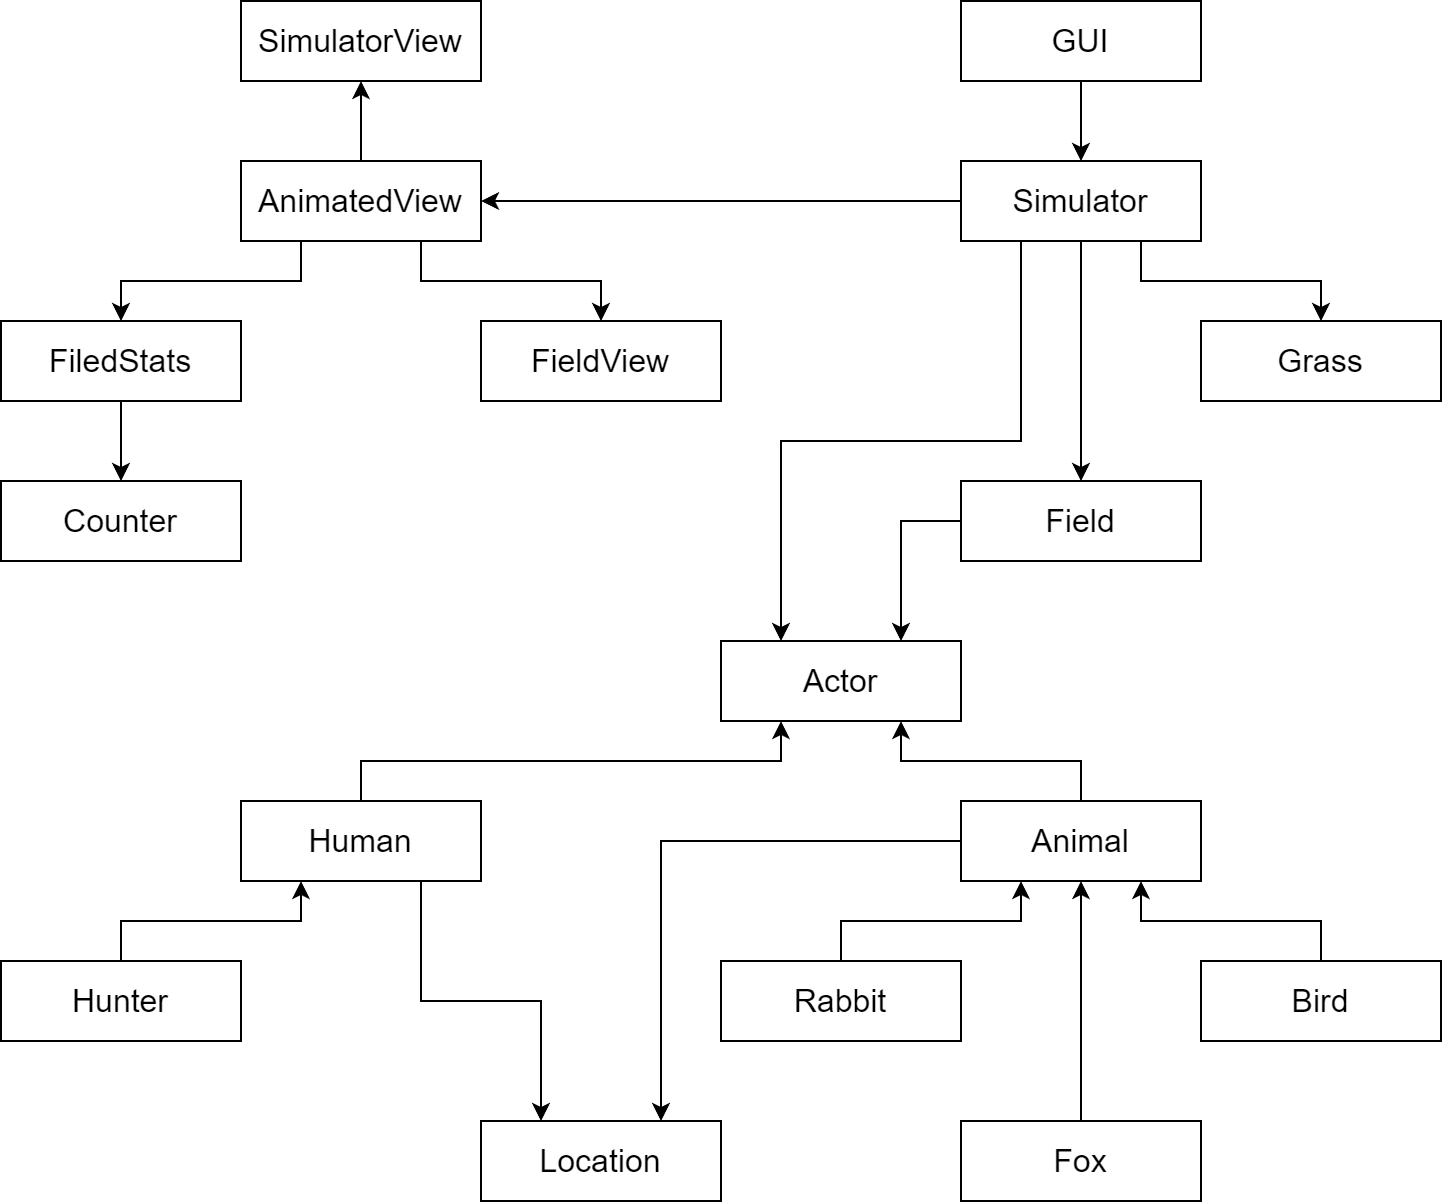
\includegraphics[width=.65\textwidth]{brex.png}
\caption{Схема зависимостей приложения.}
\label{fig:brexSchema}
\end{figure}

После применения каждой из описанных выше стадий, фреймворк выделит потенциальные участки, относящиеся к сквозным функциональностям, присутствующим в программе. В качестве результата фреймворк генерирует диаграмму найденных связей, пример которой приведен ниже.

\begin{figure}[h]
\centering
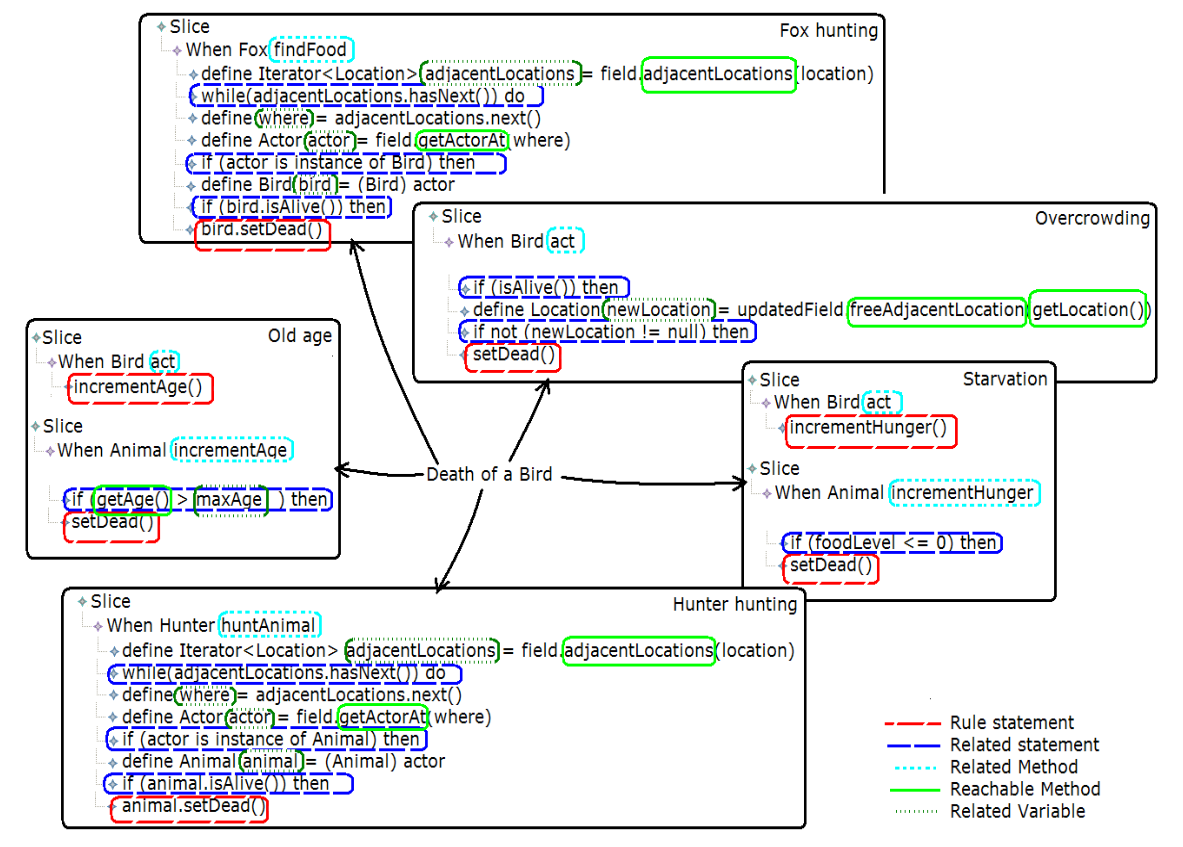
\includegraphics[width=.8\textwidth]{brex-result.png}
\caption{Результат работы фреймворка - потенциальные причины смерти птицы.}
\label{fig:brexResult}
\end{figure}

Схема на \autoref{fig:brexResult} является текстовым представлением всех условий, которые приводят к смерти птиц в данной модели. На изображении выделены различные сгенерированные бизнес-логики, контролирующие смерть птиц, которые были обнаружены фреймворком. Данный анализ может помочь установить все явные и неявные контракты приложения, однако он не решает изначальной проблемы: кодовая база все еще не модуляризована и имеет множество сквозных функциональностей. Ниже речь пойдет о том, как внедрение элементов АОП позволяет повысить модульность проекта и избежать спутывания кода.

Поскольку широкое распространение парадигма АОП получила в языке \texttt{Java}, для него были написаны многие фреймворки, привносящие элементы АОП в язык и платформу \texttt{JVM}. Популярность АОП на платформе \texttt{JVM} объясняется в том числе относительной открытостью элементов процесса сборки к расширению. Например пользователь имеет возможность встроить свои элементы логики на многих важных этапах компиляции, таких как загрузка считанного файла в виртуальную машину или построение дерева абстрактного синтаксиса. Еще одной причиной распространенности парадигмы АОП среди \texttt{Java} приложений является наличие в языке механизма аннотаций, позволяющего помечать пользовательскими данными место определения класса, функции или поля, а также место использования типа. Данные аннотации будут сохранены в бинарный класс-файл и позже могут быть считаны как компилятором, так и во время исполнения кода рантаймом виртуальной машины посредством языковых средств рефлексии. Наличие механизма аннотаций делает естественным внедрение логик, основанных на аннотировании языковых сущностей. Более того, в самом языке \texttt{Java} определены несколько встроенных аннотаций, которые также можно считать зачатками аспектно-ориентированности в языке. Например аннотация $@Deprecated$ означает, что сущность, помеченная этой аннотацией больше не является поддерживаемой, и ее использование должно быть ограничено. Встречая использование сущности, помеченной этой аннотацией, компилятор будет генерировать соответствующее предупреждение, что будет приводить к падению процесса сборки при должных настройках проекта.

\begin{lstlisting}[language=Java, caption=Пример использования аннотации \texttt{Deprecated}, label=lst:javaDeprecated]
/**
 * @deprecated
 * explanation of why it was deprecated
 */
@Deprecated
static void deprecatedMethod() { }
\end{lstlisting}

Выше в \autoref{lst:javaDeprecated} приведен пример использования аннотации \texttt{Deprecated}. Любое дальнейшее использование метода \texttt{deprecatedMethod} будет сопровождаться предупреждением от компилятора.

Примером того, как бинарная манипуляция может помочь с достижением модуляризации аспектов может служить следующий пользовательский сценарий, полученный из промышленной кодовой базы. Чтобы обеспечить выполнение требований к безопасности, при сборке приложения под определенное окружение разработчик может захотеть убедиться, что перед любым применением некоторого набора функций будет вызываться служебная процедура, проверяющая все необходимые для обеспечения безопасности условия. Исходя из описанного выше, наивная имплементация подобной логики приведет к пересечению аспекта, отвечающего за обеспечение безопасности, с основной функциональностью приложения. Чтобы избежать этого и обеспечить модульность контракта безопасности используется следующая АОП архитектура, основанная на применении пользовательских аннотаций бинарной манипуляции.

\begin{lstlisting}[language=Java, caption=Пример решения задачи замены функции в месте вызова при помощи АОП, label=lst:callSiteAOP]
    /*
     * Declaration of the annotation that will be used to specify
     * safe wrappers for the library API.
     */
    @interface CallSiteReplacement {
        String targetClass();
        String methodName();
    }
    /* Class that is responsible for providing safe wrappers for the library API. */
    public class ApiControl {
        /*
         *Presence of this annotation means that we need to replace all calls to
         * the method `foo` from the class `com.xxx.Api` with the calls to
         * `ApiControl.WrapApiFoo`.
         */
        @CallSiteReplacement(targetClass="com.xxx.Api", methodName="foo");
        public static void wrapApiFoo(target: com.xxx.Api, ...) {
            /* Logic that ensures safe use of the `foo` API. */
        }
    };
\end{lstlisting}

Рассмотрим \autoref{lst:callSiteAOP}. В нем приведен пример того, как может быть реализована АОП архитектура, обеспечивающая вызов безопасной обертки для библиотечного метода \texttt{foo} класса \texttt{com.xxx.Api}. Класс \texttt{ApiControl} реализует функционал, проверяющий все необходимые параметры для безопасного вызова конкретных функций библиотеки. Каждый метод этого класса - это безопасная обертка одной из библиотечных функций. Аспектом в даной архитектуре является механизм замены мета вызова на безопасный при определенных параметрах сборки. Данный аспект, как и каждый, состоит из двух частей - точки соединения (join point) и совета (advice). Точка соединения - это точка в выполняемой программе, где следует применить совет. В данном случае точкой соединения будет являться каждая конкретная инстанциация аннотации \texttt{CallSiteReplacement}. В ней указаны два параметра: \texttt{targetClass} и \texttt{methodName}. Они определяют то, вызовы какого метода должен быть заменены на безопасную обертку. Советом же в данной схеме будет являться логика преобразования бинарного файла, находящая все функции, аннотированные аннотацией \texttt{CallSiteReplacement}, и заменяющая все вызовы методов, указанных в аргументах аннотации на вызов аннотированной функции. Ниже в  \autoref{lst:callSiteAOP2} приведен пример того, как выглядит код до и после применения описанных выше трансформаций.

\begin{lstlisting}[language=Java, caption=Демонстрация работы аспекта, label=lst:callSiteAOP2]
/* Before AOP. */
public class MyClass {
    public static void main() {
        com.xxx.Api api = GetApi();
        api.foo(...);
    }
};

/* After AOP. */
public class MyClass {
    public static void main() {
        com.xxx.Api api = GetApi();
        ApiControl.wrapApiFoo(api, ...);
    }
};
\end{lstlisting}

В результате применения данной схемы реализации удается достигнуть модуляризации логики замены вызова функции на ее обертку, что избавляет кодовую базу от сквозных функциональностей, тем самым улучшая качество кода и стоимость его поддержки.

\subsection{Рефлексия}

Рефлексия - это способность системы или программы инспектировать и модифицировать собственную структуру во время исполнения. Для языка \texttt{Java} это означает изменение поведения загруженных классов, интерфейсов, методов и полей во время исполнения. Данная возможность позволяет программному обеспечению динамически изменять собственное поведение в зависимости от параметров времени исполнения. Применение рефлексии в производстве облегчает разработку и дальнейшую поддержку программ, предоставляя средства для гибкой интеграции со сторонними кодовыми базами и для отделения логики конфигурирования поведения программы в зависимости от параметров окружения в во время исполнения.

\begin{figure}[h]
\centering
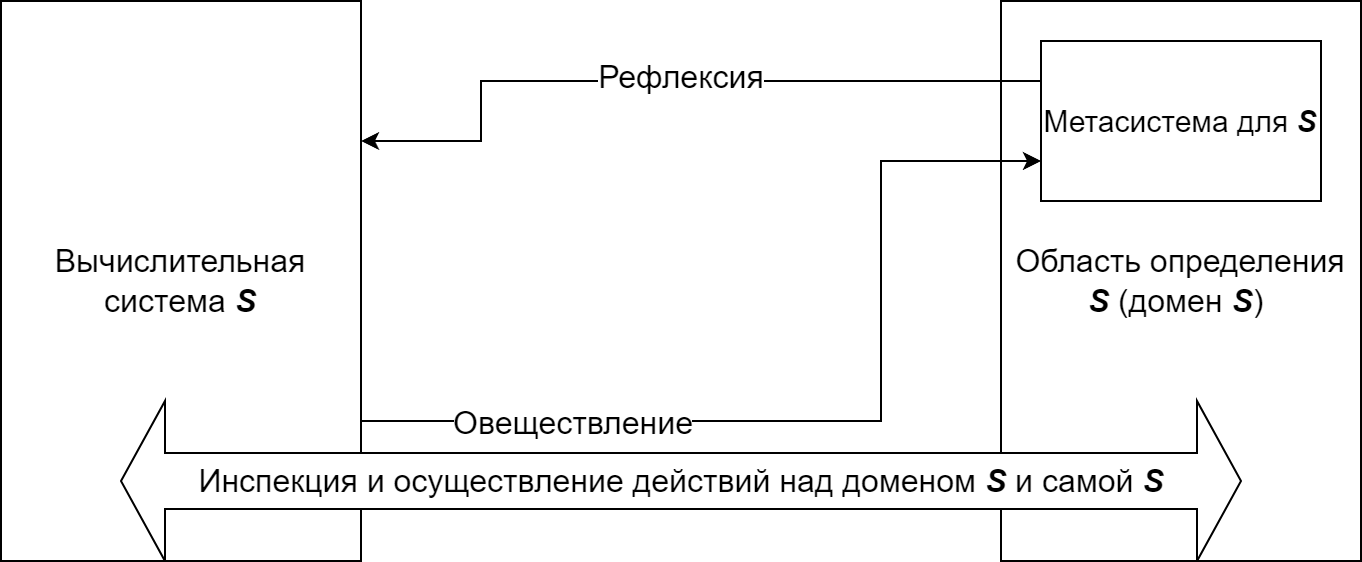
\includegraphics[width=.7\textwidth]{reflect.png}
\caption{Рефлексивная вычислительная система.}
\label{fig:reflectionScheme}
\end{figure}

Как показано на \autoref{fig:reflectionScheme}, в своем наиболее общем виде рефлексивная система может быть определена как система, удовлетворяющая следующим требованиям. Во-первых, система \texttt{S} должна иметь в своем домене собственное представление, называемое метасистемой. Это представление должно быть доступно для инспекции и манипуляции. Во-вторых, существует связь между системой \texttt{S} и ее представлением. Любое изменение в системе должно приводить к соответствующему изменению в метасистеме, и наоборот \cite{javaReflection}. То есть система \texttt{S} должна быть овеществлена (reified) в свое представление прежде чем метасистема может начать оперировать. Затем метасистема инспектирует и манипулирует системой средствами рефлексии используя представление \texttt{S}. Данные связи отражены подписанными стрелками на \autoref{fig:reflectionScheme}.

Несмотря на потенциальные плюсы полноценной рефлексии, многие решения, предоставляемые стандартными библиотеками весьма ограничивают пользователя в возможности изменения объектов или же вовсе запрещают модификацию. Подобное решение связано с тем, что неконтролируемое использование возможностей рефлексии может привести к коду, о поведении которого очень сложно судить, что только ухудшает качество разработки. Однако существуют сценарии, в которых подобный подход наоборот приводит более прозрачной логике проекта. Примером такого сценария может служить задача отслеживания изменения состояния. Для достижения этой цели наиболее естественным решением будет является переопределение операции доступа к состоянию в рантайме, нежели чем написание отдельной программы, проходящейся по всем методам бинарного класс-файла и инструментирующей все операции доступа к состоянию. Помочь с имплементацией этого подхода может бинарная манипуляция. Существует множество фреймворков, использующих бинарную манипуляцию для имплементации расширений к языку. Примером подобного фреймворка может служить \texttt{Kava}, подробнее о которой будет рассказано в \autoref{sec:Chapter2}.

\subsection{Конфигурация и оптимизация}

Бинарная манипуляция также широко применяется для имплементации пользовательских оптимизаций и конфигурации параметров кода в зависимости от параметров сборки. Как правило, такие пользовательские настройки делаются при помощи препроцессора, который способен менять структуру приложения на уровне исходного кода. Однако многие высокоуровневые языки не обладают доступным пользователю препроцессором. В качестве альтернативного решения зачастую используются фреймворки бинарной манипуляции, позволяющие изменить результирующий бинарный код аналогично тому, как препроцессор меняет исходный. Примером подобной пользовательской настройки может служить \autoref{lst:debug}

\begin{lstlisting}[language=Java, caption=Пример использования класса с конфигурацией проекта, label=lst:debug]
/* Configuration class. */
public class Configuration {
    public static Boolean debug = False;
}

/* User written code. */
public static class MyClass {
    public static void foo() {
        if (Configuration.debug) {
            /* Debug logic. */
        }
        /* Release logic. */
    }
}
\end{lstlisting}

Для того, чтобы убрать из поставляемого пользователю бинарного файла все следы кода, используемого для отладки, авторы библиотек пишут свои собственные расширения к компилятору, использующие бинарную манипуляцию. Целью данного преобразования является удаления \texttt{true} ветки всех подобных условных операторов.

\begin{lstlisting}[language=Java, caption=Результат работы преобразования, label=lst:debug]
/* After binary manipulations. */
public static class MyClass {
    public static void foo() {
        /* Release logic. */
    }
}
\end{lstlisting}

Данный подход является очень дешевым и распространенным способом настройки поведения приложения, хоть и не дает всех плюсов, обеспечиваемых парадигмой АОП.

\subsection{Актуальность}

Выше была показана востребованность инструментов бинарной манипуляции. Действительно, многие бизнес-логики больших и даже средних компаний построены на применении описанных техник, особенно в таких языках как \texttt{Java} и \texttt{Kotlin}, где подобные инструменты имеют долгую историю развития. Поэтому, чтобы оставаться конкурентноспособной, любая платформа, намеревающаяся выйти на рынок разработки мобильных приложений, обязана предоставить свои средства для решения проблем интероперабельности компонент, поддержки принципов АОП и анализа программ посредством рефлексии или инспекции бинарных файлов. Более того, решение должно быть разработано с учетом всех особенностей платформы и предоставлять свои преимущества по сравнению с конкурирующими. В данной работе были рассмотрены дизайн и реализация библиотеки для манипуляции бинарными файлами многоязыковой платформы. Были рассмотрены особенности проектирования, связанные с необходимостью поддержки бинарных файлов, полученных из исходных файлов на разных языках, проведено сравнение с существующими решениями на других платформах, а также показано, как разработанный инструмент способен эффективно решать задачи, встречающиеся в реальных бизнес-логиках.

\newpage
